\subsection{Controllers for z$_{\mathrm{I}}$ Direction}
The controller along the $z_{\mathrm{I}}$ direction is designed using a cascade approach.
%As in the case of the controller in the $x_{\mathrm{I}}$ and $y_{\mathrm{I}}$ directions, a cascade approach is chosen for the $z_{\mathrm{I}}$ direction.

The transfer function to control the velocity is shown in \autoref{eq:FinalLinearEquationZ}. It is obtained from the translational linearized block diagram seen in \autoref{fig:TranslationalLinearModelBlockDiagram}. The sum of the motor rotational speeds is the input and the velocity in the $z_{\mathrm{I}}$ is the output. %From \autoref{eq:FinalLinearEquationZ}, %with the corresponding translational linearized block diagram in \autoref{fig:TranslationalLinearModelBlockDiagram}, the linear transfer function for the z-direction is readily obtained.
%
\begin{flalign}
  \frac{\dot{z}_{\mathrm{I}}}{\omega_{\mathrm{sum}}} &= \frac{ \frac{1}{4}\ (-2 k_{\mathrm{th}})\ \overline{\omega}_{sum} }{ m s }  \label{eq:linearTransferFunctionZ}
\end{flalign}

\begin{where}
  \va{\dot{z}_{\mathrm{I}}}{is the velocity in the $z_{\mathrm{I}}$ direction}{}
  \va{\omega_{\mathrm{sum}}}{is the sum of velocities to be controlled}{}
  \va{\overline{\omega}_{\mathrm{sum}}}{is the sum of rotor velocities in equilibrium}{}
\end{where}

This transfer function has a pole in zero and a negative gain, which means that the root locus on increasing gain drives the system into the right half plane and makes it unstable. This implies a controller with negative gain. As in the case of the other translational controllers, an integral term is added to reduce the effect of input disturbances.
 
The root locus of the system, which contains two poles in zero, branches along the imaginary axis. To avoid oscillations, the two loci are attracted by the use of a zero, placed on the left real axis as seen in \autoref{fig:rootLocusOfZwithPI}.

\begin{figure}[H]
	\centering
	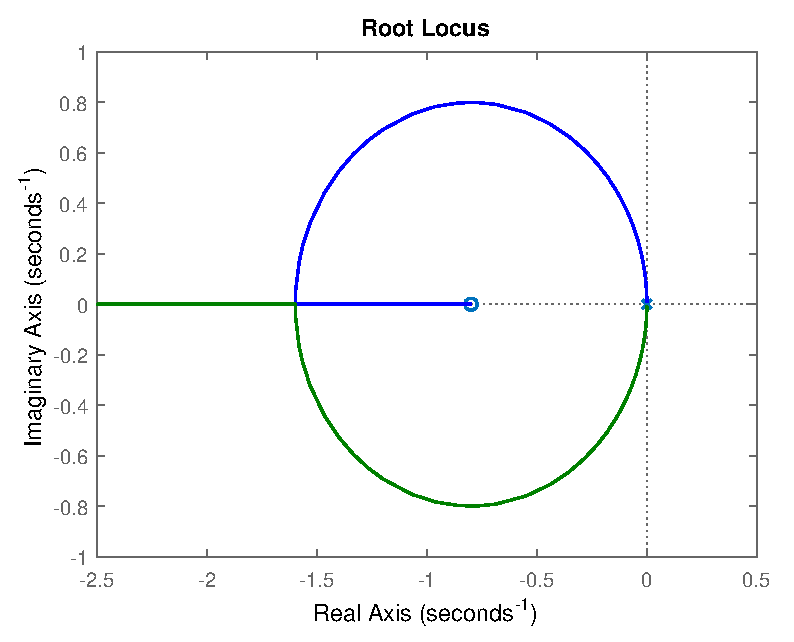
\includegraphics[width=.6\textwidth]{figures/rootLocusOfZwithPI.pdf}
	\caption{Root locus of the system with PI control. The zero is placed in $s=-0.8$}
	\label{fig:rootLocusOfZwithPI}
\end{figure}

The zero is placed and the gain is scaled to achieve the smallest rise time without reaching the limits of the control action. The zero is placed in -0.8 on the real axis and the gain of the controller is -280.

The final expression for the velocity controller is
%
\begin{flalign}
    C_{\dot{x}_{\mathrm{I}}}(s)&= -280 \frac{s+0.8}{s} \label{eq:Czdot}
\end{flalign}
%
The position controller for $z_{\mathrm{I}}$ direction is designed using the same procedure as for $x_{\mathrm{I}}$ and $y_{\mathrm{I}}$. As in these cases, the position transfer function is an integrator.
%
\begin{flalign}
    G_{z_{\mathrm{I}}}(s)&=\frac{z_{\mathrm{I}} (s)}{\dot{z}_{\mathrm{I}} (s)}=\frac{1}{s}  \label{eq:Gz}
\end{flalign}

The proportional gain is chosen so that the bandwidth of the position loop is three times lower than that of the velocity loop. This is seen in the close loop Bode of the velocity control loop. This defines it to be \SI{1}{rad s^{-1}}. Since the pant already has this bandwidth, the gain is just 1 in this case.
%
\begin{figure}[H]
    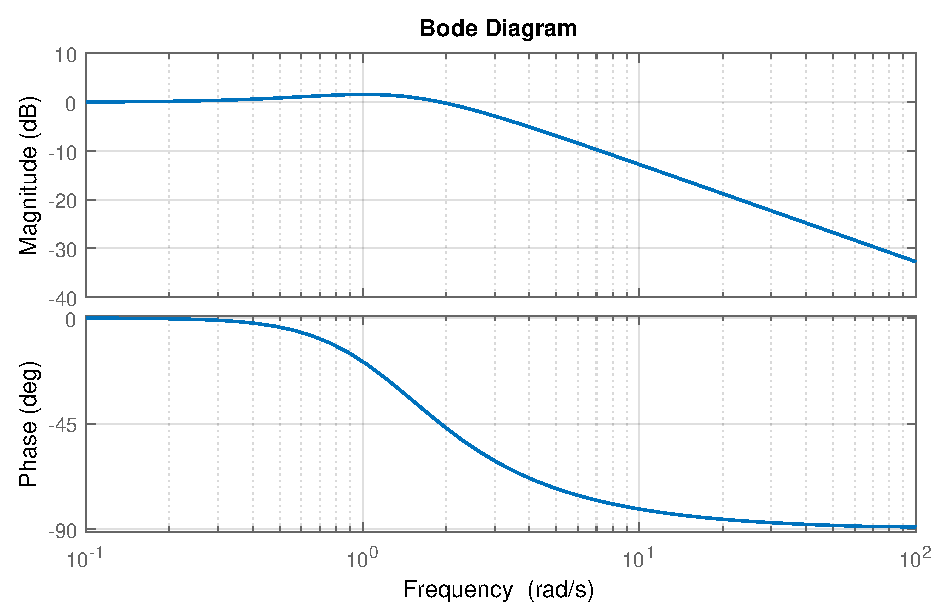
\includegraphics[scale=.7]{figures/bodeVelocityZ}
    \centering			
    \captionof{figure}{Closed loop Bode of the plant and the controller for the $z_{\mathrm{I}}$ translational velocity.} 
    \label{fig:bodeVelocityZ}
\end{figure}
%
The expression for the $z_{\mathrm{I}}$ position controller is shown in \autoref{eq:Cz}.
%
\begin{flalign}
    C_{z_{\mathrm{I}}}(s)&= 1\label{eq:Cz}
\end{flalign}


% The step response of the linear system with the PI controller is seen on \autoref{fig:stepOfZwithPI}.
%
%\begin{figure}[H]
%	\centering
%	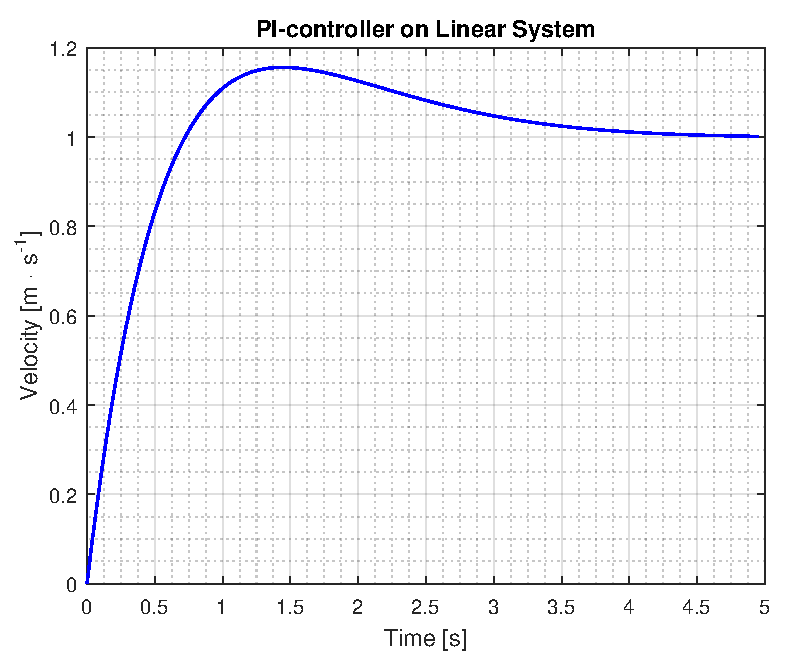
\includegraphics[width=.6\textwidth]{figures/stepOfZwithPI.pdf}
%	\caption{Step response of the linear system with PI control.}
%	\label{fig:stepOfZwithPI}
%\end{figure}
%


%
%If a gain of $-200$ is applied, the controller will bring the velocity to \SI{1}{m \cdot s^{-1}} in approximately \SI{2}{s}, see \autoref{fig:ZstepPcontrolLinear}.
%
%\begin{figure}[H]
%    \centering
%    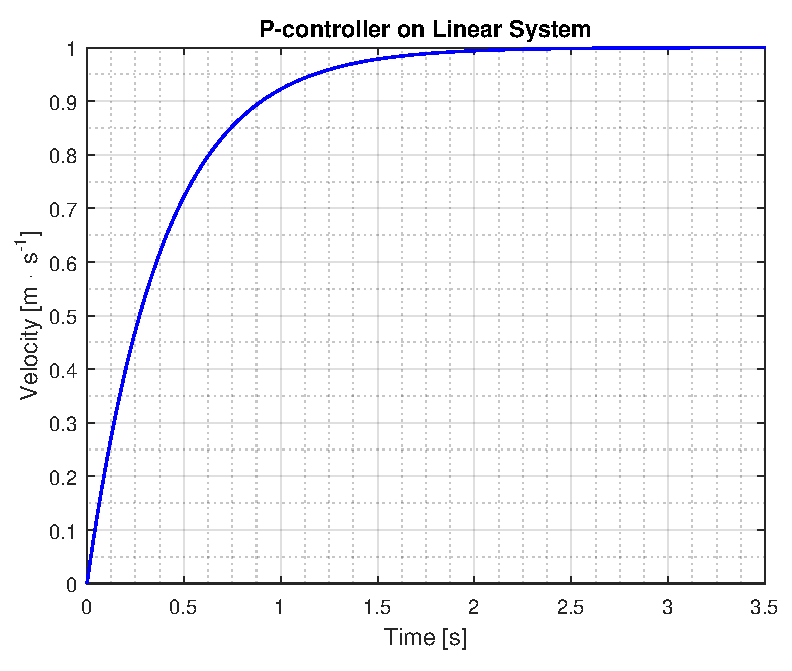
\includegraphics[width=.6\textwidth]{figures/ZstepPcontrolLinear.pdf}
%    \caption{Step response of the linear transfer function with a P-controller with a gain of $-200$.}
%    \label{fig:ZstepPcontrolLinear}
%\end{figure}
%
%%However a P-controller does not account for input disturbances, and neither does the integrator in the plant. Therefore, if the equilibrium speed of the rotors has an offset under some flight conditions, this error will not be accounted for.
%To see this effect, the P-controller is tested on the nonlinear model with an added difference of \SI{5}{rad \cdot s^{-1}} in each of the four needed equilibrium speeds in the model. The simulation is seen below in \autoref{fig:ZstepPcontrolNonlinear}, where the reference input is subjected to a step of \SI{1}{m \cdot s^{-1}}, however, the velocity stabilizes instead at \SI{0.9}{m \cdot s^{-1}}, revealing a steady state error.
%
%\begin{figure}[H]
%    \centering
%    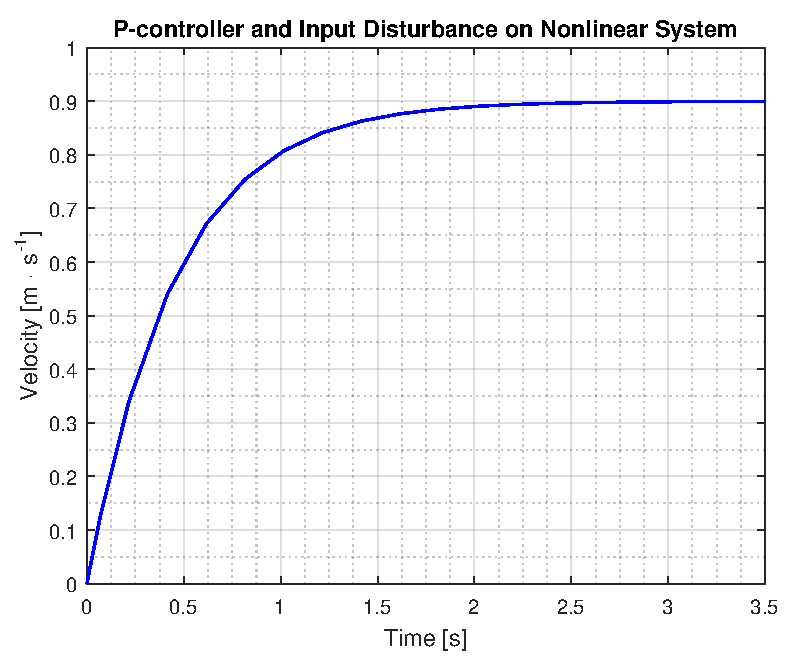
\includegraphics[width=.6\textwidth]{figures/ZstepPcontrolNonlinear.pdf}
%    \caption{Step response of the nonlinear transfer function with a P-controller with a gain of $-200$.}
%    \label{fig:ZstepPcontrolNonlinear}
%\end{figure}
%%
%%In order to remove the steady state error an integrator is introduced to the controller. 
%
%
%
